%\documentclass[iop]{emulateapj}
\documentclass[preprint]{aastex}
%\documentclass[12pt, onecolumn]{emulateapj}
%\documentstyle[aas2pp4,natbib209]{article}

\usepackage{tikz}
\usepackage{natbib}
\usepackage{amsmath}

\usetikzlibrary{shapes.geometric, arrows}
\usetikzlibrary{fit}

\tikzstyle{hyper} = [circle, text centered, draw=black]%, fill=blue!30]
\tikzstyle{param} = [circle, text centered, draw=black]%, fill=green!30]
\tikzstyle{data} = [circle, text centered, draw=black, line width=2pt]%, 
fill=red!30]
%\tikzstyle{hyper} = [trapezium, trapezium left angle=70, trapezium right 
angle=110, minimum width=1cm, minimum height=0.5cm, text centered, draw=black, 
fill=green!30]
%\tikzstyle{param} = [rectangle, minimum width=1cm, minimum height=0.5cm, text 
centered, draw=black, fill=green!30]
%\tikzstyle{data} = [diamond, minimum width=1cm, minimum height=1cm, text 
centered, draw=black, fill=red!30]
%\tikzstyle{eqn} = [rectangle, minimum width=1cm, minimum height=0.5cm, text 
centered, draw=black]%, fill=green!30]
%\tikzstyle{latent} = [diamond, minimum width=1cm, minimum height=0.5cm, text 
centered, draw=black]%, fill=green!30]
\tikzstyle{arrow} = [thick,->,>=stealth]

\newcommand{\myemail}{aimalz@nyu.edu}
\newcommand{\textul}{\underline}

\shorttitle{A Probabilistic Approach to the Redshift Distribution Function}
\shortauthors{Malz and Hogg}

\begin{document}

\title{A Fully Probabilistic Approach to the Redshift Distribution Function}

\author{A.I. Malz\altaffilmark{1}}
\email{aimalz@nyu.edu}

\author{D.W. Hogg\altaffilmark{1}}
\email{david.hogg@nyu.edu}

\altaffiltext{1}{New York University Center for Cosmology and Particle Physics}

\begin{abstract}
Photometric redshift probability distribution functions are rapidly replacing 
redshift point estimates as data products of photometric galaxy surveys.  
Though there is not yet agreement on the best way to derive such data products, 
they are most commonly stacked to obtain an estimate of the redshift 
distribution function necessary for weak gravitational lensing calculations and 
reduced to point estimates in calculations of more complicated statistics.  
This work challenges that paradigm and proposes a mathematically consistent 
technique motivated by fundamental probability theory in which a probabilistic 
graphical model elucidates the relation of interim photometric redshift 
posteriors to a full posterior distribution over relevant physical parameters.  
The approach is applied to the one-point statistic of the redshift distribution 
function $N(z)$, sampled by Monte Carlo-Markov Chain procedures and validated 
on synthetic data.  It is demonstrated that this method improves accuracy 
compared to popular alternatives such as stacking and conversion of photometric 
redshift probability distributions to point estimates of redshift.
\end{abstract}

\keywords{photo-z}

\clearpage
\section{Introduction}
\label{sec:intro}

The era of precision cosmology, heralded by weak gravitational lensing 
tomography and baryon acoustic oscillation peak measurements, has been enabled 
by photometric estimation of redshifts previously accessible only by time- and 
resource-intensive spectroscopic confirmation.  However, photometric redshifts 
(photo-zs) are susceptible to a number of errors, particularly their inherent 
noisiness due to the coarseness of photometric filters, systematic errors 
introduced by observational techniques, and catastrophic errors in which 
galaxies of one type at one redshift are mistaken for galaxies of another type 
at a different redshift.  In addition to these limitations in accuracy, there 
is also the matter of precision; photo-zs are often reported with error bars 
derived without inclusion of all systematic errors, including the different 
selection effects between the magnitude-spaces of galaxies for which photo-zs 
are desired and galaxies with spectroscopically confirmed redshifts used to 
calibrate photo-z estimators.

Since their conception \citep{Baum1962}, much effort has been dedicated to 
improving photo-zs, though they are still most commonly obtained by a maximum 
likelihood estimator (MLE) based on libraries of galaxy spectral energy 
distribution (SED) templates with conservative approaches to error estimation.  
Recent work has focused on identifying and removing catastrophic outliers when 
using photo-zs for inference.  \citep{Gorecki2014}  Sophisticated Bayesian 
techniques and cutting-edge machine learning methods have been employed to 
improve precision \citep{Carliles2010} and accuracy \citep{Sadeh2015}. 

An alternative to point estimates of photo-zs is redshift probability 
distribution function estimation, in which rather than an MLE point estimate, 
the full posterior probability (or likelihood) function of the redshift of a 
galaxy is reported.  \citep{Budavari2009}  This option is favorable because it 
contains more potentially useful information than a point estimate while 
addressing the issues with systematics and precision.  Photo-z probability 
distribution functions are not without their own weaknesses, the foremost of 
which are the computation time and storage space necessary to calculate and 
record them for large galaxy surveys  \citep{CarrascoKind2014} and the method 
used to derive them.

There is not yet consensus on the best way to obtain photo-z probability 
distributions and many techniques have been proposed and tested in the 
literature.  An extension of the Bayesian photometric redshift (BPZ) method of 
\citet{Benitez2000} that produces posterior probability distributions (as 
opposed to a selection of local maxima) from an SED template library has been 
employed.  \citep{Hildebrandt2012, Kelly2014, Lopez-Sanjuan2015}  Photo-z 
posterior probability distributions have also been obtained by a variety of 
trustworthy data-driven approaches in the literature: $k$-nearest neighbor 
algorithms with \citep{Ball2008} and without \citep{Sheldon2012} inclusion of 
photometric measurement errors, neural networks \citep{Bonnett2015a}, 
self-organizing maps \citep{CarrascoKind2014a}, and prediction tree and random 
forest classification techniques \citep{Carliles2010, CarrascoKind2013}.  

Photo-z probability distributions have been produced by completed surveys 
\citep{Hildebrandt2012, Sheldon2012} and will be produced by upcoming surveys 
\citep{LSSTScienceCollaboration2009, CarrascoKind2014a}.  Though their 
potential to improve estimates of physical parameters is tremendous, photo-z 
posterior probability distributions have seldom been used to infer physical 
parameters.  Furthermore, no implementation of inference with photo-z posterior 
distributions has been presented with a mathematically consistent methodology.  
The goal of this paper is to clearly present and validate a technique for the 
use of photo-z posterior distributions in inference.  For simplicity, we 
consider only one-point statistics relevant to cosmology, though future work 
will extend this methodology to higher-order statistics.

The redshift distribution function $N(z)$ serves as an ideal statistic upon 
which to demonstrate such an approach, in large part because it has been the 
subject of inference using photo-z probability distributions before.  
\citep{Sheldon2012, Kelly2014, Benjamin2013, Bonnett2015a, Viironen2015, 
Asorey2016}  $N(z)$ for observed galaxies can be used to validate survey 
selection functions used in generation of realistic mock catalogs used for many 
purposes.  \citep{Norberg2002}  The redshift density function $n(z)$, derived 
from the redshift distribution function $N(z)$, is also necessary for 
calculations of two-point correlation functions of weak lensing shear and 
counting statistics that are directly used to probe cosmological parameters.  
\citep{Masters2015}

\clearpage
\section{Method}
\label{sec:meth}

It is best to begin with a general description of the problem at hand.  Let us 
consider a survey of $J$ galaxies $j$, each with photometric data 
$\vec{d}_{j}$; thus the entire survey over some solid angle $\Omega$ produces 
the ensemble of photometric magnitudes (or colors) and their associated 
observational errors $\{\vec{d}_{j}\}_{J}$.  Each galaxy $j$ has a redshift 
$z_{j}$ that we would like to learn; redshift is a parameter in this case.  The 
distribution of the ensemble of redshifts $\{z_{j}\}_{J}$ may be described by 
the hyperparameters defining the redshift distribution function $N(z)$ that 
would like to find.  This situation may be considered to be a probabilistic 
generative model, illustrated by the directed acyclic graph of Fig. 
\ref{fig:flow}.  

\begin{figure}
\vspace{0.5cm}
\begin{center}
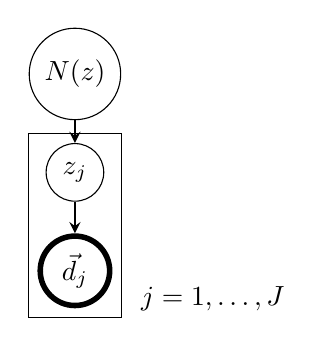
\begin{tikzpicture}[node distance=1cm]

\node (nz) [hyper] {$N(z)$};
\node (z) [param, below of=nz,yshift=-0.25cm] {$z_{j}$};
\node (mags) [data, below of=z,yshift=-0.25cm] {$\vec{d}_{j}$};
\node (survey) [draw=black,fit={(mags.west)(z.north)(mags.south)(mags.east)}] 
{};
\node [xshift=1.75cm,yshift=0.25cm] at (survey.south) {$j=1,\dots,J$};

\draw [arrow] (nz) -- (z);
\draw [arrow] (z) -- (mags);

\end{tikzpicture}
\caption{This directed acyclic graph illustrates a hierarchical model.}
\label{fig:flow}
\end{center}
\end{figure}

The redshift distribution function $N(z)$ shown in Eq. \ref{eq:distribution} 
gives the number of galaxies per unit redshift, effectively quantifying 
evolution in the number of galaxies.  \citep{Menard2013}  According to Eq. 
\ref{eq:density}, the redshift distribution function $N(z)$ is related to the 
redshift density function $n(z)$, which gives the number of galaxies per unit 
redshift per unit volume in redshift-space spherical coordinates.  The redshift 
density function provides additional information about cosmology via the rate 
of expansion over redshift.

\begin{eqnarray}
\label{eq:distribution}
N(z) &=& \frac{dN}{dz}
\end{eqnarray}

\begin{eqnarray}
\label{eq:density}
n(z) &=& \frac{dN}{dz\ d\Omega}
\end{eqnarray}

\clearpage
\subsection{Probabilistic Model}
\label{sec:prob}

We begin by parametrizing $N(z)$ in terms of $\vec{\theta}$, some set of 
parameters that define the form $N(z)$ may take in whatever basis we choose.  
At this point, these hyperparameters are quite general and may represent 
coefficients in a high-order polynomial as a function of redshift, a set of 
means and variances defining Gaussians that sum to the desired distribution, a 
set of histogram heights that describe a binned version of the redshift 
distribution function, etc.  We define a function $f_{\vec{\theta}}(z)=N(z)$ 
that transforms these hyperparameters into the redshift distribution function 
$N(z)$.

In this paper, we shall work exclusively with log-probabilities.  What we wish 
to estimate is the full posterior probability distribution of the parameters 
$\vec{\theta}$ given the data $\{\vec{d}_{j}\}_{J}$.  By Bayes' Rule, the full 
posterior $\ln[p(\vec{\theta}|\{\vec{d}_{j}\}_{J})]$ may be expressed in terms 
of the full likelihood $\ln[p(\{\vec{d}_{j}\}_{J}|\vec{\theta})]$ by way of a 
hyperprior $\ln p(\vec{\theta})$ and the probability of the data 
$\ln[p(\{\vec{d}_{j}\}_{J})]$.  The hyperprior expresses our beliefs about the 
distribution of the hyperparameters comprising $\vec{\theta}$; this is a choice 
we cannot avoid making and one which is often inspired by the results of 
previous galaxy surveys.  The probability of the data is generally unknowable, 
but the full posterior probability distribution can be probed with a quantity 
proportional to it.  The full likelihood may be expanded in terms of a 
marginalization over the redshifts as parameters, as in Eq. 
\ref{eq:marginalize}.  

\begin{eqnarray}
\label{eq:marginalize}
\ln[p(\{\vec{d}_{j}\}_{J}|\vec{\theta})] &=& \ln\left[\int\ 
p(\{\vec{d}_{j}\}_{J}|\{z_{j}\}_{J})\ p(\{z_{j}\}_{J}|\vec{\theta})\ 
d\{z_{j}\}\right]
\end{eqnarray}

We shall make two assumptions of independence in order to make the problem 
tractable; their limitations are be discussed below.  First, we take 
$\ln[p(\{\vec{d}_{j}\}_{J}|\{z_{j}\}_{J})]$ to be the sum of $J$ individual 
likelihood distribution functions $\ln[p(\vec{d}_{j}|z_{j})]$, as in Eq. 
\ref{eq:indiedat}, a result of the definition of probabilistic independence.  
Second, we shall assume the true redshifts $\{z_{j}\}_{J}$ are $J$ independent 
draws from the true $N(z)$.  Additionally, $J$ itself is a Poisson random 
variable with expected value $J'$.  The combination of these assumptions is 
given by Eq. \ref{eq:indie}  It is important to note that $\int N(z)\ dz$ is 
not constrained to equal $J'$ but instead $J$, which can be thought of as 
another parameter.  A detailed discussion of this matter may be found in 
\citet{Foreman-Mackey2014}.

\begin{eqnarray}
\label{eq:indiedat}
\ln[p(\{\vec{d}_{j}\}_{J}|\{z_{j}\}_{J})] &=& \sum_{j=1}^{J}\ 
\ln[p(\vec{d}_{j}|z_{j})]
\end{eqnarray}

\begin{eqnarray}
\label{eq:indie}
\ln[p(\{z_{j}\}_{J}|\vec{\theta})] &=& -\int\ f_{\vec{\theta}}(z)\ dz +  
\sum_{j=1}^{J}\ \ln[p(z_{j}|\vec{\theta})]
\end{eqnarray}

Applying Bayes' Rule, we may now combine terms to obtain Eq. 
\ref{eq:posterior}.  

\begin{eqnarray}
\label{eq:posterior}
\ln[p(\vec{\theta}|\{\vec{d}_{j}\}_{J})] &\propto& \ln[p(\vec{\theta})]\ -\int 
f_{\vec{\theta}}(z)\ dz + \sum_{j=1}^{J}\ \ln\left[\int\ p(\vec{d}_{j}|z_{j})\ 
p(z_{j}|\vec{\theta})\ dz_{j}\right]
\end{eqnarray}

Eq. \ref{eq:posterior} still contains the photo-z likelihoods 
$\ln[p(\vec{d}_{j}|z_{j})]$ unaddressed since Eq. \ref{eq:marginalize} that are 
in this case inaccessible.  Both empirical and data-driven methods for 
obtaining photo-z probability distributions effectively assign to each galaxy's 
photometry $\vec{d}_{j}$ both a redshift $z_{j}$ and some nuisance parameters 
determined by an interim prior $\vec{\theta}^{0}$, encapsulated by the reported 
interim photo-z posteriors $\ln[p(z_{j}|\vec{d}_{j},\vec{\theta}^{0})]$.  The 
interim prior may be thought of as an initial guess for $\vec{\theta}$ 
including some parameters defining intrinsic galaxy spectra and instrumental 
effects inspired by the generative model for photometry from the redshift 
distribution functions. (See \citet{Benitez2000} for more detail.)  In the case 
of estimating $N(z)$ photometrically it is common to use $\vec{\theta}^{0}$ 
corresponding to $N(z)$ derived from some different, spectroscopically 
confirmed sample or from a cosmological simulation.  For statistical purposes, 
we would like any interim prior to be uninformative, but this is rarely 
achievable.  

Since we only have access to interim photo-z posteriors, we must be able to 
write the full posterior distribution for the desired hyperparameters in terms 
of the interim photo-z posteriors rather than the likelihoods of Eq. 
\ref{eq:posterior}.  The method outlined here is valid regardless of how the 
interim photo-z posteriors are calculated so the many approaches to producing 
photo-z probability distributions will not be discussed; though the matter is 
outside the scope of this paper, various methods have been presented in the 
literature. \citep{Sheldon2012, Ball2008, CarrascoKind2013, CarrascoKind2014a}  
However, we will need an explicit statement of this interim prior for whatever 
method is chosen to produce the interim photo-z posteriors.  To perform the 
necessary transformation from likelihoods to posteriors, we follow the 
reasoning of \citet{Marshall2015}.  Let us consider the probability of the 
parameters conditioned on the data and an interim prior and rewrite the 
problematic likelihood of Eq. \ref{eq:posterior} as Eq. \ref{eq:trick}.  

\begin{eqnarray}
\label{eq:trick}
p(\vec{d}_{j}|z_{j}) &=& p(\vec{d}_{j}|z_{j})\ 
\frac{p(z_{j}|\vec{d}_{j},\vec{\theta}^{0})}{p(z_{j}|\vec{d}_{j},\vec{\theta}^{0
})}
\end{eqnarray}

Once the interim prior $\vec{\theta}^{0}$ is explicitly introduced, we may 
expand the denominator according to Bayes' Rule to get Eq. \ref{eq:expand}.  
Because there is no direct dependence of the data upon the hyperparameters, we 
may again expand the term $p(\vec{d}_{j}|z_{j},\vec{\theta}^{0})$ to obtain Eq. 
\ref{eq:indterm}.  Canceling the undesirable likelihood terms 
$p(\vec{d}_{j}|z_{j})$ and $p(\vec{d}_{j}|\vec{\theta}^{0})$ yields Eq. 
\ref{eq:cancel}.  We put this all together to get the full posterior 
probability distribution of Eq. \ref{eq:final}.

\begin{eqnarray}
\label{eq:expand}
p(\vec{d}_{j}|z_{j}) &=& p(\vec{d}_{j}|z_{j})\ 
p(z_{j}|\vec{d}_{j},\vec{\theta}^{0})\ 
\frac{p(\vec{d}_{j}|\vec{\theta}^{0})}{p(z_{j}|\vec{\theta}^{0})\ 
p(\vec{d}_{j}|z_{j},\vec{\theta}^{0})}
\end{eqnarray}

\begin{eqnarray}
\label{eq:indterm}
p(\vec{d}_{j}|z_{j}) &=& p(\vec{d}_{j}|z_{j})\ 
p(z_{j}|\vec{d}_{j},\vec{\theta}^{0})\ 
\frac{p(\vec{d}_{j}|\vec{\theta}^{0})}{p(z_{j}|\vec{\theta}^{0})\ 
p(\vec{d}_{j}|z_{j})\ p(\vec{d}_{j}|\vec{\theta}^{0})}
\end{eqnarray}

\begin{eqnarray}
\label{eq:cancel}
p(\vec{d}_{j}|z_{j}) &=& 
\frac{p(z_{j}|\vec{d}_{j},\vec{\theta}^{0})}{p(z_{j}|\vec{\theta}^{0})}
\end{eqnarray}

\begin{eqnarray}
\label{eq:final}
\ln[p(\vec{\theta}|\{\vec{d}_{j}\}_{J})] &\propto& \ln[p(\vec{\theta})]-\int 
f_{\vec{\theta}}(z)\ dz + \sum_{j=1}^{J}\ \ln\left[\int\ 
p(z_{j}|\vec{d}_{j},\vec{\theta}^{0})\ 
\frac{p(z_{j}|\vec{\theta})}{p(z_{j}|\vec{\theta}^{0})}\ dz_{j}\right]
\end{eqnarray}

The argument of the integral in the posterior of Eq. \ref{eq:final} depends 
solely on knowable quantities (and those we must assume) and can be calculated 
for a given set of interim photo-z posterior distribution functions 
$\{p(z_{j}|\vec{d}_{j},\vec{\theta}^{0})\}_{J}$ and the interim prior 
$\vec{\theta}^{0}$ upon which their determination was based, noting the 
relation of Eq. \ref{eq:params}.  Since we cannot know constant of 
proportionality, we sample the desired distribution 
$\ln[p(\vec{\theta}|\{\vec{d}_{j}\}_{J})]$ using Monte Carlo-Markov chain 
(MCMC) methods.  

\begin{eqnarray}
\label{eq:params}
p(z_{j}|\vec{\theta}) &=& \frac{f_{\vec{\theta}}(z_{j})}{\int\ 
f_{\vec{\theta}}(z_{j})\ dz_{j}}
\end{eqnarray}

To be clear, the following assumptions must be made in order to apply this 
method:

\begin{enumerate}
\item Photometric measurements of galaxies are independent Poisson draws from 
the set of all galaxies such that Eqs. \ref{eq:indiedat} and \ref{eq:indie} 
hold.
\item We take the reported interim photo-z posterior distribution functions to 
be accurate estimates of the true photo-z posterior distribution functions and 
assume we are given the interim prior used to produce them.
\item We must assume a hyperprior constraining the underlying probability of 
the hyperparameters comprising $\vec{\theta}$.
\end{enumerate}

These assumptions have known limitations.  First, the photometric data are not 
a set of independent measurements; the data are correlated not only by the 
conditions of the experiment under which they were made but also by redshift 
covariances resulting from physical processes governing underlying galaxy 
spectra and their relation to the redshift distribution function.  Second, the 
reported interim photo-z posterior distributions may not be trustworthy; there 
is not yet agreement on the best technique to obtain photo-z probability 
distributions, and the interim prior may not be appropriate or even known to us 
as consumers of interim photo-z posteriors.  Third, the hyperprior may be quite 
arbitrary and poorly motivated if the underlying physics is complex.

\clearpage
\subsection{Competing Methods}
\label{sec:sheldon}

It will be desirable to compare the result of this method to the estimates of 
the hyperparameters obtained by two popular alternatives used in the 
literature, known as stacking and point estimation.   These have been compared 
to one another by \citet{Hildebrandt2012}, \citet{Benjamin2013}, and 
\citet{Asorey2016}.

Stacking directly calculates the full posterior for the entire dataset using 
the interim photo-z posteriors for each galaxy according to Eq. \ref{eq:stack}. 
 \citep{Lima2008}  It must be noted here that Eq. \ref{eq:stack} is not 
mathematically valid.  (See \citet{Hogg2012} for a complete discussion.)  

\begin{eqnarray}
\label{eq:stack}
f_{\hat{\theta}}(z) &=& \sum_{j=1}^{J}\ p(z_{j}|\vec{d}_{j},\vec{\theta}^{0})
\end{eqnarray}

Point estimation, converts the interim photo-z posteriors 
$p(z_{j}|\vec{d}_{j},\vec{\theta}^{0})$ into delta functions with all 
probability at a single redshift.  Some variants of point estimation choose 
this single redshift to be that of maximum a posteriori (MAP) probability 
$argmax[p(z_{j}|\vec{d}_{j},\vec{\theta}^{0})]$ or the expected value of 
redshift $\int z_{j}\ p(z_{j}|\vec{d}_{j},\vec{\theta}^{0})\ dz_{j}$.  Stacking 
these modified interim photo-z posteriors leads to the marginalized MAP 
estimator and the marginalized $E[z]$ estimator.

A final estimator of the hyperparameters is the maximum marginalized likelihood 
estimator (MMLE), the value of $\hat{\theta}$ maximizing the likelihood given 
by Eq. \ref{eq:mmle}.

\begin{eqnarray}
\label{eq:mmle}
\ln[p(\{\vec{d}_{j}\}_{J}|\vec{\theta})] \propto -\int\ f_{\vec{\theta}}(z)\ 
dz+\sum_{j=1}^{J}\ln\left[\int\ 
\exp\left[\ln[p(z_{j}|\vec{d}_{j},\vec{\theta}^{0})]+\ln[f_{\vec{\theta}}(z)]-\l
n[f_{\vec{\theta}^{0}}(z)]\right]\ dz\right]
\end{eqnarray}

\clearpage
\section{Experiments}
\label{sec:exp}

We ran several tests of this approach to demonstrate its validity and usage 
using a procedure outlined in this section.  In Sec. \ref{sec:mock} we describe 
the method by which sets of simulated interim photo-z posteriors 
$\{\ln[p(z_{j}|\vec{d}_{j})]\}_{J}$ are generated in all test cases.  In Sec. 
\ref{sec:data} we describe the real datasets used for further tests.  In Sec. 
\ref{sec:mcmc} we describe the algorithm used to compute the full posterior 
distribution $\ln[p(\vec{\theta}|\{\vec{d}_{j}\}_{J})]$.  In Sec. 
\ref{sec:diag} we outline the measures used to evaluate the performance of the 
method, including the competing methods with which our results will be compared.

\subsection{Mock Data}
\label{sec:mock}

To generate mock interim photo-z posteriors, we first produce a catalog of true 
redshifts.  We choose a physically-motivated $p^{0}(z)$ defining the general 
shape of $N(z)$ over a specified redshift range $[z_{min},z_{max}]$.  Here we 
shall set it to a weighted sum of truncated Gaussians chosen to impose 
recognizably recoverable features on the true $N(z)$.  The true survey size $J$ 
is a Poisson random variable distributed about a target survey size of $J'$.  
Next we take $J$ samples of $z\sim p^{0}(z)$ to obtain the true redshift 
catalog $\{z_{j}^{0}\}_{J}$.  

The catalog of log photo-z posteriors $\{\ln[p(z_{j}|\vec{d}_{j})]\}_{J}$ is 
chosen to be a set of Gaussian distributions, truncated to the redshift range 
over which $N(z)$ is defined, because it is the simplest extension of the 
standard redshift point estimates with reported error bars.  To simulate the 
fact that inaccuracy increases with redshift, each Gaussian is centered at a 
redshift $z_{j}'$ separated from the true redshift $z_{j}^{0}$ by a Gaussian 
random variable $\epsilon_{j}$ selected from a distribution of mean of 0 and 
variance $v_{j}\propto(1+z_{j}^{0})^{2}$.  To simulate the fact that 
imprecision also increases with redshift, the variances of the truncated 
Gaussians are also set to $\{v_{j}\}_{J}$.

At this point we choose a parametrization of redshift space and impose a 
$K$-dimensional binning $B_{k}=[z^{B}_{k-1},z^{B}_{k}]$ on the redshift range 
from $z^{B}_{0}=z_{min}$ to $z^{B}_{K}=z_{max}$ with bin widths $\Delta_{k}$.  
All tests in this paper will be conducted with $K=35$.  We must also choose the 
parametrization of the redshift distribution function, in this case 
$f_{\vec{\theta}}(z)=\ln[\vec{\theta}]$.  We next define the elements of 
$\vec{\theta}$ to be log top-hat functions where the hyperparameters 
$\theta_{k}$ comprising $\vec{\theta}$ take values equal to 
$\ln[\int_{z_{k-1}}^{z_{k}}\ f_{\vec{\theta}}(z)\ dz]$.  By default we choose a 
flat distribution as the interim prior.

To obtain the desired interim photo-z posteriors, we simply normalize such that 
each interim photo-z posterior integrates to unity and has components 
proportional to the integral of the product of the interim prior and the 
Gaussian redshift posterior over each bins.  A random sampling of such interim 
redshift posteriors with $K=35$ is shown in Fig. \ref{fig:nullpzs}.

\begin{figure}
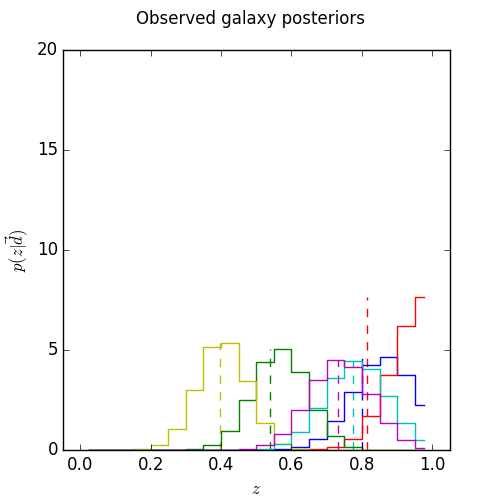
\includegraphics[width=0.5\textwidth]{null/samplepzs.png}
\caption{Several examples of individual photo-z posterior distributions are 
shown in colors.  The solid lines indicate the true redshift and the dotted 
lines indicate the shifted redshift used as the center of the Gaussian 
distribution.}
\label{fig:nullpzs}
\end{figure}

\subsection{BOSS Data}
\label{sec:data}

We also test this method on subsets of the published interim photo-z posteriors 
of SDSS III DR 10.  A sampling of the provided interim photo-z posteriors of 
dimension $K=35$ for $z_{min}=0.3$ and $z_{max}=1.4$ is shown in Fig. 
\ref{fig:datapzs}.  The interim prior used for this set of interim redshift 
posteriors is the reweighted estimator of $N(z)$ of \citet{Sheldon2012}.

\begin{figure}
%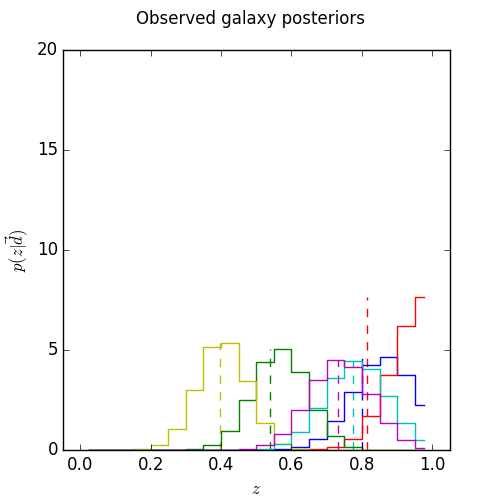
\includegraphics[width=0.5\textwidth]{null/samplepzs.png}
\caption{}
\label{fig:datapzs}
\end{figure}

\clearpage
\subsection{Implementation}
\label{sec:mcmc}

The testing procedure is implemented in \texttt{Python}.  The code takes as 
input a \texttt{csv} file containing the basis for the parametrization of 
redshift space, a specification of the interim prior $\vec{\theta}^{0}$, and a 
catalog of $J$ interim photo-z log-posteriors 
$\{\ln[p(B_{j}|\vec{d}_{j},\vec{\theta}^{0})]\}_{J}$ each of length $K$ in the 
given basis.  The assumed hyperprior distribution is described in Sec. 
\ref{sec:prior}.

The \texttt{emcee} implementation of the Metropolis-Hastings algorithm is 
applied to sample the full posterior of Eq. \ref{eq:final}.   
\citep{Foreman-Mackey2013}   At each iteration $i$, a proposal distribution 
$\vec{\theta}^{i}$ generated from this hyperprior distribution and evaluated 
for acceptance to or rejection from the desired posterior distribution 
according to the algorithm outlined below.  

\begin{enumerate}
\item \label{it:randsamp} Randomly sample the hyperprior $\ln[p(\vec{\theta})]$ 
to generate a proposal $\vec{\theta}^{i}$.
\item Calculate the log posterior as in Eq. \ref{eq:final} to produce a 
quantity proportional to $\ln[p(\vec{\theta}^{i}|\{\vec{d}_{j}\}_{J})]$.
\item Calculate 
$a=\ln[p(\vec{\theta}^{i}|\{\vec{d}_{j}\}_{J})]-\ln[p(\vec{\theta}|\{\vec{d}_{j}
\}_{J})]$.
\item If $a\geq0$, set and record $\vec{\theta}=\vec{\theta}^{i}$.\\
If $a<0$, select a random number $n$ from the uniform distribution between 0 
and 1.
\begin{enumerate}
\item If $n<\exp[a]$, set and record $\vec{\theta}=\vec{\theta}^{i}$.
\end{enumerate}
\item Check if the threshold condition has been achieved; if not, return to 
Step \ref{it:randsamp}.
\end{enumerate}

Here, the threshold condition is defined in terms of sub-runs of $I_{0}$ 
accepted samples.  When the variance of the log probabilities is less than the 
change in median log probability over the sub-run, the burn-in period is 
considered complete.  When this occurs, an additional number of sub-runs equal 
to the number $I'$ of sub-runs consumed by the burn-in period are completed 
such that the total number of accepted samples is $I=2I'$.  

The input/output format chosen for this work is \texttt{HDF5} because of its 
efficiency for large amounts of data.  The resulting output is a set of $I$ 
ordered \texttt{hickle} files (should I use \texttt{FITS}?) enumerated by 
$\rho$ containing the state information after each sub-run.  The state 
information includes $\frac{I_{0}}{t}$ actual samples $\vec{\theta}^{i}$ for a 
pre-specified chain thinning factor and their full posterior probabilities 
$p(\vec{\theta}^{i}|\{\vec{d}_{j}\}_{J})$ as well as the autocorrelation times 
and acceptance fractions calculated for each element of $\vec{\theta}$ over the 
entire sub-run.  These two summary statistics are described in Sec. 
\ref{sec:diag}, along with the proper use of the other outputs in interpreting 
the results of the code.

\clearpage
\subsubsection{Prior}
\label{sec:prior}

The method of Sec. \ref{sec:mcmc} involves the assumption of a prior 
distribution on the hyperparameters in $\vec{\theta}$.  The prior chosen here 
is a multivariate normal distribution with mean $\vec{\theta}^{0}$ equal to the 
interim prior and covariance $\textul{\Sigma}$ inspired by one used in Gaussian 
processes, given by Eq. \ref{eq:priorcov}.  This choice is made to permit draws 
from this prior distribution to produce shapes similar to that of the true 
$\tilde{\theta}$.  Here, the parameters of this covariance matrix are set to 
the small numbers $q=?$, $e=?$, and $t=?$.  We adapt the full posterior of Eq. 
\ref{eq:final} to the binning of redshift space chosen in Sec. \ref{sec:mock}.

\begin{eqnarray}
\label{eq:priorcov}
\Sigma_{a,b} &=& q\ \exp[-\frac{e}{2}\ (\bar{z}_{a}-\bar{z}_{b})^{2}]\ +\ t\ 
v_{a,b}
\end{eqnarray}

The sampler is initialized with $2K$ walkers each with a value chosen from a 
Gaussian distribution of identity covariance around a sample from the 
hyperprior distribution.  An example of such samples from the prior are shown 
in Fig. \ref{fig:nullprior}.

\begin{figure}
%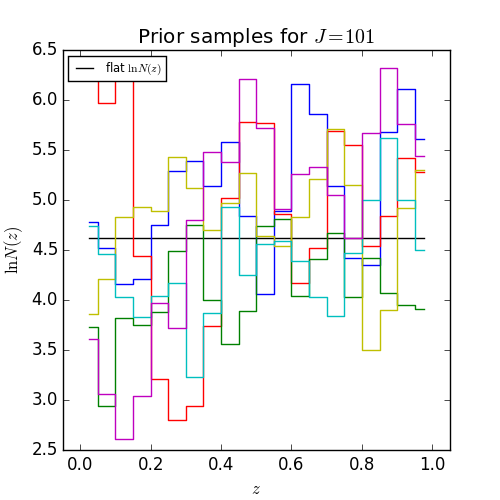
\includegraphics[width=0.5\textwidth]{null/priorsamps.png}
\caption{}
\label{fig:nullprior}
\end{figure}

\clearpage
\subsection{Diagnostics}
\label{sec:diag}

The results of the computation described in Sec. \ref{sec:mcmc} are evaluated 
on the basis of several diagnostics measures, briefly described below.

%\clearpage
\subsubsection{Autocorrelation Time}
\label{sec:acorr}

The autocorrelation time is effectively a measure of the convergence rate of 
the method and can be described as the expected number of iterations necessary 
to accept a sample independent of the current sample.  A sampler that converges 
faster will have a smaller autocorrelation time, and smaller autocorrelation 
times are preferable because it means fewer iterations are wasted on 
non-independent samples when independent samples are desired.  Typically, the 
autocorrelation time decreases with successive iterations through a burn-in 
phase before leveling out.  See \citet{Foreman-Mackey2013} for a more complete 
exploration of the autocorrelation time.

%\clearpage
%\subsubsection{Posterior Probability Evolution}
%\label{sec:probs}
%
%In order to evaluate the duration of the burn-in phase, it can be helpful to 
examine the evolution of the posterior probability of each accepted set of 
parameters.  Though the probability associated with the initial values will 
likely be quite low, the probability should improve for subsequent accepted 
parameter values.  As with the diagnostics of Secs. \ref{sec:acorr} and 
\ref{sec:afrac}, the posterior probability of samples will asymptotically 
approach some more favorable value with more iterations.  The burn-in phase may 
be identified as the number of iterations necessary before the probabilities 
are sufficiently close to the value at which they level out.  Samples accepted 
during the burn-in phase are typically discounted from analysis.  
%
%The posterior probabilities for the samples may also be compared to the 
posterior obtained by the competing approaches discussed in Sec. 
\ref{sec:sheldon}; higher posterior probabilities indicate a better fit than 
the alternative.  The distribution of the posterior probabilities of the 
samples may also be an informative measure of performance.
%
%\clearpage
%\subsubsection{Parameter Evolution}
%\label{sec:params}
%
%An intuitive diagnostic used here is the evolution of the parameter values 
themselves.  We would like to see each walker move throughout parameter space 
near the true value rather than remaining stationary or in some small region 
around another value.  We can visually inspect the parameter values each walker 
takes over successive iterations to ensure that the walkers are not being 
caught in small regions of parameter space far from the true parameter values.  
%
%Inspection of the parameter evolution can also be a good test of the 
appropriateness of the prior distribution; if the covariance matrix of the 
prior distribution is too restrictive, the walkers will not be able to sample 
parameter values far from their initialization.  
%
%\clearpage
\subsubsection{Parameter Values}
\label{sec:samps}

Sampled values of hyperparameters are also visually inspected for accuracy when 
the true values are known.  When using simulated data where a true value is 
known, the sampler is performing well if samples are near the true value.  The 
distribution of the parameter values can also reveal how well the samples fit 
the data.  If there is a strongly peaked distribution of values for a 
parameter, it ought to peak close to the true value if we are to conclude that 
the sampler is successful; if the distribution is broad, it may reflect 
inherent uncertainty in inferring the hyperparameters.

%\clearpage
\subsubsection{Summary Statistics}
\label{sec:stats}

Beyond visual inspection of samples, we calculate summary statistics to 
quantitatively compare different estimators' precision and accuracy.  Since 
MCMC samples of hyperparameters are Gaussian distributions, we can quantify the 
breadth of the distribution for each hyperparameter using the standard 
deviation regardless of whether the true values are known.  Three measures of 
accuracy of hyperparameter samples $\vec{\theta}^{i}$  have been considered 
here for the cases where the true values are known.  

%The likelihood ratio comparing the samples to competing methods may be 
calculated for a sample $\vec{\theta}^{i}$ as in Eq. \ref{eq:llr}.  Values of 
$A$ greater than 0 indicate the sampler fits the data better than the competing 
method.  The log posterior probabilities of Sec. \ref{sec:probs} are used to 
obtain the log likelihoods via Eq. \ref{eq:logpost} and the sample values 
themselves are used to calculate the prior probability term according to Eq. 
\ref{eq:llr-how}; the difference between the log posteriors and the log prior 
probability is the log likelihood, and the difference between log likelihoods 
is the log likelihood ratio.  Because the sampler produces many samples of 
parameter values, the log likelihood ratio for the sampler versus each 
alternative is a distribution of values.
%
%\begin{eqnarray}
%\label{eq:llr}
%A(\vec{\theta}^{i}) &=& 
-2\ln[\tilde{p}(\{\vec{d}_{j}\}_{J}|\vec{\theta}_{test})]+2\ln[\tilde{p}(\{\vec{
d}_{j}\}_{J}|\vec{\theta}^{i})]
%\end{eqnarray}
%
%\begin{eqnarray}
%\label{eq:llr-how}
%\ln[\tilde{p}(\{\vec{d}_{j}\}_{J}|\vec{\theta})] &=& 
\ln[\tilde{p}(\vec{\theta}|\{\vec{d}_{j}\}_{J})]-\ln[p(\vec{\theta})]
%\end{eqnarray}

%In simulated cases where the true parameter values are known, we calculate the 
Kullback-Leibler divergence (KLD), given in Eq. \ref{eq:kl} which measures a 
distance between parameter values $\vec{\theta}^{a}$ and $\vec{\theta}^{b}$ 
that is invariant under changes of variables.  We note that $KL_{ab}\neq 
KL_{ba}$, so both must be calculated.  In simulated tests, one of 
$\vec{\theta}^{a}$ and $\vec{\theta}^{b}$ are the true value and the other is 
the value produced by one of the methods in question.  For the sampler, the KLD 
is calculated for all samples and shown as a distribution of KLD values.
%
%\begin{eqnarray}
%\label{eq:kl}
%KL_{ab} &=& \sum_{k=1}^{K}\ \exp[\theta_{k}^{a}]\ 
\ln\left[\frac{\theta_{k}^{a}}{\theta_{k}^{b}}\right]\ \Delta_{k}
%\end{eqnarray}

%The mean squared error of samples relative to the true value may also be 
calculated.  Both the variance $\sigma^{2}$ and $\chi^{2}$ statistics are 
calculated for the accepted samples and for the competing methods relative to 
the true value in the simulated tests.
%

\clearpage
\section{Validation Tests}
\label{sec:valid}

Here we motivate and present the results of several informative tests.  The 
code was tested on several simulated datasets each of size $J_{0}=10,000$.  The 
fiducial experiment of Sec. \ref{sec:null} was generated by code following the 
procedure given in Sec. \ref{sec:mock}.  Six other cases vary the shapes of the 
interim photo-z posteriors (Sec. \ref{sec:unc}), the true redshift distribution 
function (Sec. \ref{sec:fake}), and the interim prior (Sec. \ref{sec:interim}). 
 Two additional cases with real data described in Sec. \ref{sec:data} are also 
considered.

\clearpage
\subsection{Fiducial Case}
\label{sec:null}

For the fiducial experiment, we precisely follow the procedures outlined in 
Sec. \ref{sec:mock} and Sec. \ref{sec:mcmc}.  Fig. \ref{fig:null-samp} shows 
some random sample values and the $1\sigma$ errors of the aggregate of samples 
as well as the true value of $N(z)$ and the estimators derived from stacking 
and marginalized likelihood maximization.  Fig. \ref{fig:null-comp} compares 
the mean of the sample values to alternative estimators as well as the truth.

\begin{figure}
%\includegraphics[width=0.5\textwidth]{null/samps.pdf}
\caption{The smooth, black curve shows the true $N(z)$ for this test, a sum of 
Gaussians described in Sec. \ref{sec:mock}.  The flat, gray line is the interim 
prior used to generate the interim photometric redshift posteriors.  The 
colored step functions are random samples from the full posterior.  $1\ \sigma$ 
errors about the mean from the posterior are plotted in gray.  It can be 
plainly seen that the samples are an excellent estimator of the truth with the 
true values falling within the error bars.}
\label{fig:null-samp}
\end{figure}

\begin{figure}
%\includegraphics[width=0.5\textwidth]{null/comps.pdf}
\caption{The smooth, black curve shows the true $N(z)$ for this test, a sum of 
Gaussians described in Sec. \ref{sec:mock}.  The flat, gray line is the interim 
prior used to generate the interim photometric redshift posteriors.  The thick 
black step function is the mean of the samples.  The dotted line is the result 
of stacking, and the dashed line is the result of marginalized likelihood 
maximization.  It can be seen that the mean of the samples is a better 
estimator of the true distribution; stacking overestimates $N(z)$ at the tails 
and underestimates $N(z)$ at the peaks, and marginalized likelihood 
maximization is unstable.}
\label{fig:null-comp}
\end{figure}

In the fiducial case, hierarchical inference preserves features in the redshift 
distribution function, whereas stacking tends to smear them out.  Methods using 
point estimates of redshift also perform well because of the simplicity of the 
form of the interim photo-z posteriors.

\clearpage
\subsection{Uncertain interim photo-z posteriors}
\label{sec:unc}

In the following two tests, we aim to simulate more realistic interim photo-z 
posteriors by modifying the procedure of Sec. \ref{sec:mock} to introduce 
imprecision and inaccuracy that increase noisily with the true redshift, as is 
seen in observed photometric redshifts.

\subsection{Noisy interim photo-z posteriors}
\label{sec:noisy}

Several factors contribute to photometric redshifts' increased uncertainty with 
redshift.  As redshift increases, galaxies sharing luminosity are dimmer, 
driving up photometric errors by way of counting statistics.  The galaxy sample 
at higher redshifts also changes, meaning the generation of the photometric 
redshift posterior based on an SED template library or a 
spectroscopically-confirmed training is more likely to be inappropriate, 
leading to broader components.

This test case simulates imprecision in interim photometric redshift posteriors 
by introducing one change in the steps of Sec. \ref{sec:mock}.  After the 
shifted redshifts $z'_{j}$ are chosen, the variance of the Gaussian describing 
the shape of the photo-z posterior is chosen to not be the same $v_{j}$ but 
rather a random variable $v_{j}'$ drawn from a Gaussian of mean $v_{j}\propto 
1+z_{j}$ and variance $v_{j}^{2}$ such that the width of the Gaussian noisily 
increases with redshift.  Some interim redshift posteriors from such a test are 
shown in Fig. \ref{fig:noisypzs}.  The rest of the steps in Sec. \ref{sec:mcmc} 
are then followed precisely.

\begin{figure}
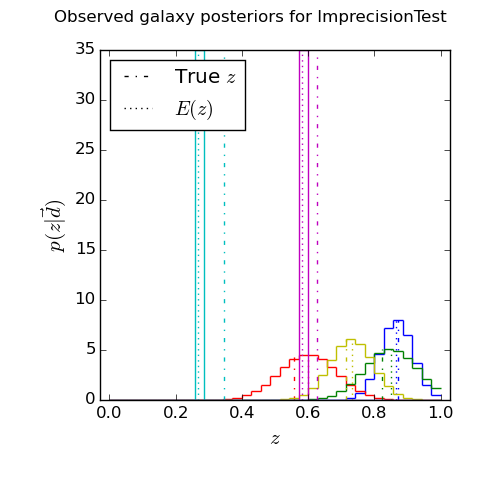
\includegraphics[width=0.5\textwidth]{sigma/samplepzs.png}
\caption{Several examples of noisified individual photo-z posterior 
distributions are shown in colors.  The solid lines indicate the true redshift 
and the dotted lines indicate the shifted redshift used as the center of the 
Gaussian distribution.  Note that the widths of the Gaussians vary randomly 
over the samples.}
\label{fig:noisypzs}
\end{figure}

Fig. \ref{fig:noisy-samp} shows random sample values and their $1\sigma$ errors 
as well as the true value of $N(z)$.  The mean of the sample values is compared 
to the results of stacking in Fig. \ref{fig:noisy-comp}.

\begin{figure}
%\includegraphics[width=0.5\textwidth]{sigma/samps.pdf}
\caption{}
\label{fig:noisy-samp}
\end{figure}

\begin{figure}
%\includegraphics[width=0.5\textwidth]{sigma/comps.pdf}
\caption{}
\label{fig:noisy-comp}
\end{figure}

When the interim photo-z posteriors are more complicated hierarchical inference 
compares more favorably against stacking and point estimators.   Stacking 
results in more severe loss of features than in the fiducial case for data 
affected by noise and misclassification.  

\clearpage
\subsubsection{Multimodal interim photo-z posteriors}
\label{sec:multi}

In this test, we aim to simulate more realistic interim photo-z posteriors by 
modifying the procedure of Sec. \ref{sec:mock} to introduce inaccuracy that 
causes catastrophic photo-z errors.  Catastrophic photo-z errors arise from a 
degeneracy in the space of galaxy SEDs and redshifts, wherein a galaxy of one 
SED type at one redshift has photometry indistinguishable from a galaxy of 
another SED type at another redshift.  To simulate this case, multimodal 
interim photo-z posteriors will be considered.

To achieve this goal we introduce another change in Sec. \ref{sec:mock}.  Here, 
the redshift posteriors are sums of Gaussians of the form of those tested in 
Sec. \ref{sec:noisy}.  Each galaxy is assigned a number $R_{j}$ of Gaussian 
elements to be summed, chosen randomly from $1,\dots,K$.  The true redshift of 
each galaxy $z_{j}^{0}$ is used to generate to $R_{j}$ Gaussian elements with 
means $\{\{z_{j}^{r_{j}}\}_{R_{j}}\}_{J}$ and standard deviations 
$\{\{v_{j}'^{r_{j}}\}_{R_{j}}\}_{J}$.  Some examples of the multimodal interim 
photo-z posteriors are shown in Fig. \ref{fig:multipzs}.  

\begin{figure}
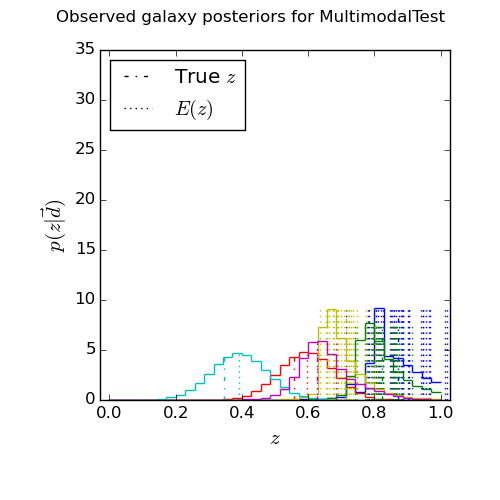
\includegraphics[width=0.5\textwidth]{multi/samplepzs.png}
\caption{Several examples of individual photo-z posterior distributions are 
shown in colors.  The solid lines indicate the true redshift and the dotted 
lines indicate the shifted redshifts used as the centers of the Gaussian 
components.  Note that the number of components increases with the true 
redshift and higher redshifts are more likely to be multimodal.}
\label{fig:multipzs}
\end{figure}

Fig. \ref{fig:multi} shows the mean sample values and their $1\sigma$ errors as 
well as the true value of $N(z)$ and the results of stacking and both point 
estimates.

\begin{figure}
%\includegraphics[width=0.5\textwidth]{multi/samps.png}
\caption{}
\label{fig:multi-samp}
\end{figure}

\begin{figure}
%\includegraphics[width=0.5\textwidth]{multi/comps.png}
\caption{}
\label{fig:multi-comp}
\end{figure}

When the interim photo-z posteriors are more complicated hierarchical inference 
compares more favorably against stacking and point estimators.   Stacking 
results in more severe loss of features than in the fiducial case for data 
affected by noise and misclassification.  

\clearpage
\subsection{Toy Model $N(z)$}
\label{sec:fake}

We test the sampler in a case of a highly unrealistic but strongly featured 
true $N(z)$.  This is done to show that the sampler works even in extreme and 
unanticipated conditions.  Here we modify the procedure of Sec. \ref{sec:mock}. 
 Instead of sampling the true distribution $p(z|\vec{\theta}')$, we sample a 
narrow Gaussian.  The rest of Sec. \ref{sec:mock} is followed precisely.  Sec. 
\ref{sec:mcmc} is followed without alteration.  Fig. \ref{fig:toy-samp} shows 
some samples from the posterior as compared to the true $N(z)$ and Fig. 
\ref{fig:toy-comp} compares the mean of the posterior samples to the results of 
stacking and marginalized likelihood maximization.

\begin{figure}
%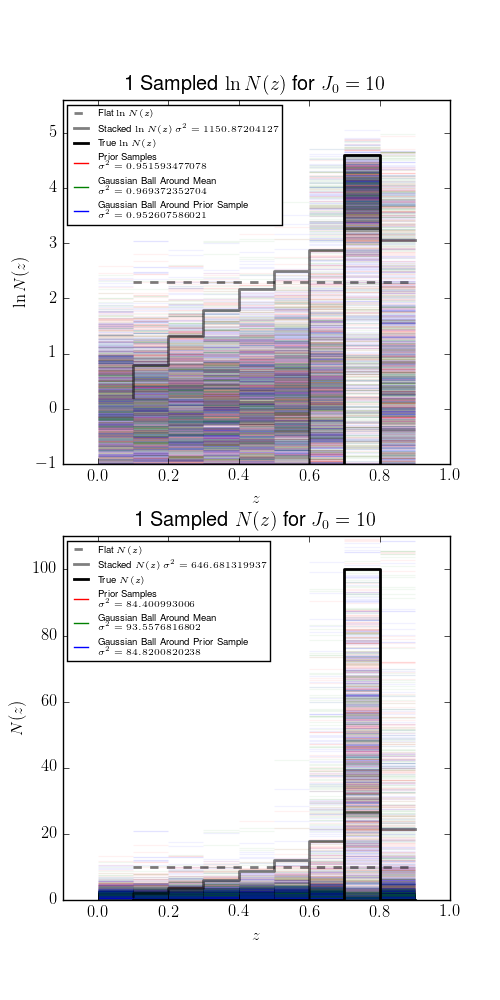
\includegraphics[width=0.5\textwidth]{toy/samps.png}
\caption{The smooth, solid, black line shows the true $N(z)$ for the toy model 
case.  The dashed line shows the result of stacking the interim photo-z 
posteriors; one can see that the distribution is broader and shorter than the 
true $N(z)$.  The dotted line shows the marginalized maximum likelihood 
estimator; one can see that the distribution is narrower than the true $N(z)$.  
Finally, the colored lines are random samples from the posterior, which trace 
the true distribution better at the tails than the stacked result and better at 
the peak than the marginalized maximum likelihood estimator.  The gray error 
bars encompass the true distribution everywhere.}
\label{fig:toy-samp}
\end{figure}

\begin{figure}
%\includegraphics[width=0.5\textwidth]{toy/comps.png}
\caption{The smooth, solid, black line shows the true $N(z)$ for the toy model 
case.  The dashed line shows the result of stacking the interim photo-z 
posteriors; one can see that the distribution is broader and shorter than the 
true $N(z)$.  The dotted line shows the marginalized maximum likelihood 
estimator; one can see that the distribution is narrower than the true $N(z)$.  
Finally, the colored lines are random samples from the posterior, which trace 
the true distribution better at the tails than the stacked result and better at 
the peak than the marginalized maximum likelihood estimator.  The gray error 
bars encompass the true distribution everywhere.}
\label{fig:toy-comp}
\end{figure}

\clearpage
\subsection{Variable Interim Prior}
\label{sec:interim}

In the following two cases we vary the interim prior used in Sec. 
\ref{sec:mock} to show that the sampler is robust to inappropriate choices of 
interim prior so long as that interim prior is known.  Typically, interim 
redshift posteriors are made with an interim prior derived from $N(z)$ in a 
previous observational study.  Since most observational studies used for this 
purpose are spectroscopically confirmed and objects for which photometric 
redshifts are relied upon make up a population that cannot be spectroscopically 
confirmed, such an interim prior is rarely appropriate.  Some efforts have been 
made to modify an observationally informed interim prior so that it is more 
representative of the data set.  \citep{Sheldon2012}  However, any interim 
prior of this kind imparts information into the interim redshift posteriors.  
Ideally, an uninformative interim prior would be used, although it may be 
complicated to compute from the covariances of the raw data.  In this test, we 
consider two obviously inappropriate interim priors and compare it to the flat 
interim prior used in previous tests according to Sec. \ref{sec:mock}.  The 
rest of the procedure of \ref{sec:mcmc} is followed precisely.

The most compelling case for hierarchical inference of the redshift 
distribution function is that of an inappropriate interim prior distribution.  
Stacking and point estimates are strongly affected by this bias introduced to 
the interim photo-z posteriors, but inference of the full posterior on the 
redshift distribution function compensates for it.  So long as the interim 
prior is known and regardless of whether it is uninformative or an accurate 
description of the data, the probabilistic approach may compensate for it and 
recover the true redshift distribution function.

\subsubsection{Low-z Favoring Interim Prior}
\label{sec:lowz}

In some cases, the interim prior is determined directly from a previous 
spectroscopic redshift survey.  Because low-redshift galaxies are more likely 
to be bright enough to be observed by such a survey, $N(z)$ determined from 
that sample will be heavily biased to low redshift galaxies.  By contrast, the 
galaxies that were unobserved in such a survey are more likely be dimmer, 
making them more likely to be at higher redshifts.  Since the interim prior is 
not compatible with our beliefs about the true redshift distribution, the 
resulting interim redshift posteriors will be inappropriate.  In this test, we 
choose an interim prior with most of its weight at low redshifts.  The results 
of the inference are shown in Figs. \ref{fig:intu-samp} and \ref{fig:intu-comp}.

\begin{figure}
%\includegraphics[width=0.5\textwidth]{int-u/samps.png}
\caption{}
\label{fig:intu-samp}
\end{figure}

\begin{figure}
%\includegraphics[width=0.5\textwidth]{int-u/comps.png}
\caption{}
\label{fig:intu-comp}
\end{figure}

\subsubsection{Mid-z Disfavoring Interim Prior}
\label{sec:midz}

One potential method for selecting an interim prior with support over the 
entire redshift range expected of the photometric survey is to sum two or more 
$N(z)$ distributions obtained from reliable photometric surveys in the past.  
This is also problematic because the sum of redshift distributions for two or 
more surveys does not reflect our beliefs about the true distribution for a 
single survey.  To simulate this, we choose an interim prior with more weight 
at high and low redshifts than for mid-range redshifts.  The results of the 
inference are shown in Figs. \ref{fig:intb-samp} and \ref{fig:intb-comp}.

\begin{figure}
%\includegraphics[width=0.5\textwidth]{int-b/samps.png}
\caption{}
\label{fig:intb-samp}
\end{figure}

\begin{figure}
%\includegraphics[width=0.5\textwidth]{int-b/comps.png}
\caption{}
\label{fig:intb-comp}
\end{figure}

\clearpage
\subsection{Data}
\label{sec:boss}

In addition to simulated tests, we also apply this method to a samples of the 
data described in Sec. \ref{sec:data}.  In these cases the true $N(z)$ is not 
known, but the fully probabilistic method presented here may still be compared 
to what is obtained by alternative approaches.

\subsubsection{Unbiased Data}
\label{sec:unbiased}

A pseudo-random sampling of the full dataset is examined to approximate the 
behavior of an unbiased galaxy survey.  The results of the inference are shown 
in Fig. \ref{fig:dataparam}.

\begin{figure}
%\includegraphics[width=0.5\textwidth]{data/samps.png}
\caption{}
\label{fig:dataparam}
\end{figure}

\subsubsection{Biased Data}
\label{sec:biased}

A pseudo-random sampling of the full dataset with a cut in $r$-band magnitude 
is examined to approximate the behavior of a biased galaxy survey with a 
magnitude limit.  The results of the inference are shown in Fig. 
\ref{fig:biasparam}.

\begin{figure}
%\includegraphics[width=0.5\textwidth]{data/samps.png}
\caption{}
\label{fig:biasparam}
\end{figure}

\clearpage
\section{Conclusion}
\label{sec:con}

This study derives and demonstrates a mathematically consistent implementation 
of inference of a one-point statistic based on interim photo-z posteriors.  

By showing that this method is effective in recovering the true redshift 
distribution function from simulated interim photo-z posteriors, this work 
supports the production of interim photo-z posteriors by upcoming photometric 
surveys such as LSST so that more accurate inference of physical parameters may 
be accessible to the scientific community.  We discourage researchers from 
co-adding interim photo-z posteriors or converting them into point estimates of 
redshift and instead recommend the use of Bayesian probability to guide the 
usage of interim photo-z posteriors in science.  We emphasize to those who 
produce interim photo-z posteriors from data that it is essential to release 
the interim prior used in generating this data product in order for proper 
inference to be conducted by consumers of this information.

The method herein developed is applicable with minimal modification to other 
one-point statistics of redshift to which we will apply this method in the 
future, such as the redshift-dependent luminosity function and weak lensing 
mean distance ratio.  Future work will also include the extension of this fully 
probabilistic approach to higher-order statistics of redshift such as the 
two-point correlation function.

%\clearpage
%\subsection{The Luminosity Function}
%\label{sec:lf}
%
%Since the redshift-dependent luminosity function $\Phi(\vec{L},z)$ is a number 
density over redshift $z$ and one other parameter, luminosity $\vec{L}$ (which 
may be a vector if not bolometric), that contributes to the same data 
$\{\vec{d}_{j}\}_{J}$ in the form of a vector of photometric magnitudes, it is 
essentially a generalization of the redshift distribution function $N(z)$ 
previously investigated here; in other words, $N(z)$ is related to 
$\Phi(\vec{L},z)$ by way of an integral over luminosity.   We may express this 
as Eq. \ref{eq:lf}, where $\Phi(\vec{L},z)$ is parametrized by hyperparameters 
that are components of $\vec{\phi}$ .
%
%\begin{eqnarray}
%\label{eq:lf}
%p(z_{j},\vec{L}_{j}|\vec{\phi}) &=& \frac{\Phi(\vec{L},z)}{\iint 
\Phi(\vec{L},z)\ d\vec{L}\ dz} = \frac{\Phi(\vec{L},z)}{\int N(z)\ dz} = 
\frac{1}{J}\ \Phi(\vec{L},z)
%\end{eqnarray}
%
%A graphical model for this problem is presented in Fig. \ref{fig:lf}.  As in 
Sec. \ref{sec:meth}, we shall outline the translation of this graphical 
representation of the probabilistic model using the same formalism.
%
%\begin{figure}
%\vspace{0.5cm}
%\begin{center}
%\begin{tikzpicture}[node distance=1cm]
%
%\node (lf) [hyper] {$\Phi(\vec{L},z)$};
%\node (z) [param, below of=lf,yshift=-0.75cm,xshift=0.5cm] {$z_{j}$};
%\node (L) [param, below of=lf,yshift=-0.75cm,xshift=-0.5cm] {$\vec{L}_{j}$};
%\node (flux) [data, below of=lf,yshift=-2cm] {$\vec{d}_{j}$};
%\node (survey) [draw=black,fit={(L.west)(z.north)(flux.south)(z.east)}] {};
%\node [xshift=1.75cm,yshift=0.25cm] at (survey.south) {$j=1,\dots,J$};
%
%\draw [arrow] (lf) -- (z);
%\draw [arrow] (lf) -- (L);
%\draw [arrow] (z) -- (flux);
%\draw [arrow] (L) -- (flux);
%
%\end{tikzpicture}
%\caption{This directed acyclic graph illustrates a hierarchical model for the 
luminosity function $\Phi(\vec{L},z)$.}
%\label{fig:lf}
%\end{center}
%\end{figure}
%
%First, we assume independence of the $J$ data points $\vec{d}_{j}$ where $J$ 
is a Poisson random variable with expected value $J_{0}$.  However, we 
acknowledge that the measurements are not independent if they are made as part 
of the same experimental design with shared equipment, not to mention the fact 
that $\vec{L}_{j}$ and $z_{j}$ are not independent of $\vec{L}_{j'\neq j}$ and 
$z_{j'\neq j}$ respectively due to the physics summarized by the luminosity 
function $\Phi(\vec{L},z)$.  However, given the assumption of independence, we 
may write the full likelihood as Eq. \ref{eq:lfind}.  
%
%\begin{eqnarray}
%\label{eq:lfind}
%p(\{\vec{d}_{j}\}_{J}|\vec{\phi}) &=& e^{-\iint \Phi(\vec{L},z)\ dL\ dz}\ 
\prod_{j=1}^{J}\ p(\vec{d}_{j}|\vec{\phi})
%\end{eqnarray}
%
%As before, we apply Bayes' Rule to relate the full likelihood to the full 
posterior in Eq. \ref{eq:lfbayes} and expand out the individual likelihood in 
terms of the parameters $\{\vec{L}_{j}\}_{J}$ and $\{z_{j}\}_{J}$ in Eq. 
\ref{eq:lfexpand}.
%
%\begin{eqnarray}
%\label{eq:lfbayes}
%p(\vec{\phi}|\{\vec{d}_{j}\}_{J}) &=& 
\frac{p(\vec{\phi})}{p(\{\vec{d}_{j}\}_{J})}e^{-\iint \Phi(\vec{L},z)\ 
d\vec{L}\ dz}\ \prod_{j=1}^{J}\ p(\vec{d}_{j}|\vec{\phi})
%\end{eqnarray}
%
%\begin{eqnarray}
%\label{eq:lfexpand}
%p(\vec{\phi}|\{\vec{d}_{j}\}_{J}) &=& 
\frac{p(\vec{\phi})}{p(\{\vec{d}_{j}\}_{J})}e^{-\iint \Phi(\vec{L},z)\ 
d\vec{L}\ dz}\ \prod_{j=1}^{J}\ \iint\ p(\vec{d}_{j}|z_{j},\vec{L}_{j})\ 
p(z_{j},\vec{L}_{j}|\vec{\phi}) dz_{j}\ d\vec{L}_{j}
%\end{eqnarray}
%
%If we are unable to access the individual likelihoods, as is in general the 
case, we will repeat the trick of using an interim prior value of 
hyperparameters $\vec{\phi}^{0}$.  This results in Eq. \ref{eq:lftrick}.
%
%\begin{eqnarray}
%\label{eq:lftrick}
%p(\vec{\phi}|\{\vec{d}_{j}\}_{J}) &=& 
\frac{p(\vec{\phi})}{p(\{\vec{d}_{j}\}_{J})}e^{-\iint \Phi(\vec{L},z)\ 
d\vec{L}\ dz}\ \prod_{j=1}^{J}\ \iint\ 
p(z_{j},\vec{L}_{j}|\vec{d}_{j},\vec{\phi}^{0})\ 
\frac{p(z_{j},\vec{L}_{j}|\vec{\phi})}{p(z_{j},\vec{L}_{j}|\vec{\phi}^{0})} 
dz_{j}\ d\vec{L}_{j}
%\end{eqnarray}

%Fig. \ref{fig:sheldon} compares the result of summing the posteriors as in Eq. 
\ref{eq:sheldon} with the result of the MCMC solutions of Eq. \ref{eq:bayes}.  
The method of \citet{Sheldon2012} underestimates the probability of observing 
low redshifts.  As one would expect, the MCMC estimate irreversibly loses some 
substructure because of the shifting error added to the simulated data.

%\begin{figure}
%\label{fig:sheldon}
%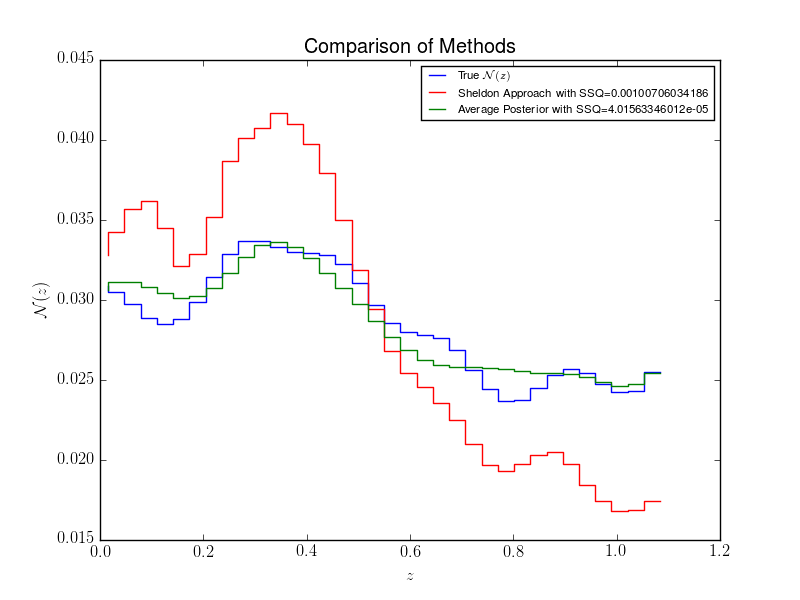
\includegraphics[width=\textwidth]{compare-sheldon.png}
%\caption{The result of applying Eq. \ref{eq:sheldon} is shown in red, the 
average accepted posterior sample from the method presented here is shown in 
blue, and $p(z)$ for the observable redshifts of Eq. \ref{eq:zshift} is shown 
in black.  The sum of squared differences between the result of each method and 
the true value are also shown; one can see that the \citet{Sheldon2012} 
approach has larger errors.}
%\end{figure}

%\acknowledgments

%\subsubsection{}
%\label{app:dumber}

%We next consider a set of $J$ galaxies representing a draw from the Poisson 
distribution $P(J_{0},J_{0})$ for $J_{0}=100$.  The galaxies share a single 
true redshift $z^{s}$ arbitrarily chosen to be the midpoint of the redshift bin 
with the largest $\theta_{k}$.  The redshift posteriors are taken to be single 
Gaussians centered at observed redshifts $z^{p}_{j}\sim 
N(z^{s},\bar{\Delta}(1+z^{s}))$ with shared variances of 
$\bar{\Delta}(1+z^{s})$. 

%\subsubsection{}
%\label{app:dumb}

%The last test case is comprised of a set of $J$ galaxies representing a draw 
from the Poisson distribution $P(J_{0},J_{0})$ for $J_{0}=1000$.  The true 
galaxy redshift bins $b_{j}=k$ from $k=1,\dots,K$ are assigned to each galaxy 
$j$ by randomly sampling the $K$ bins with weights given by the true redshift 
function of Eq. \ref{eq:truenz} as $\int_{z_{k}}^{z_{k+1}}p^{0}(z)dz$. True 
redshifts $z^{s}_{j}$ are assigned within these bins assuming a random uniform 
distribution within each bin.  The redshift posteriors are taken to be single 
Gaussians centered at observed redshifts $z^{p}_{j}\sim 
N(z^{s}_{j},\bar{\Delta}(1+z^{s}_{j}))$ with variances $\sigma_{j}\sim 
N(z^{s}_{j},\bar{\Delta}(1+z^{s}_{j}))$. 

\bibliographystyle{apj}
\bibliography{zPDF}

\end{document}